\subsection{Rendering}

W aplikacji zaimplementowano autorski system renderingu w celu zapewnienia wysokiej wydajności oraz wygody użytkowania przez użytkownika końcowego. Do realizacji tego rozwiązania wykorzystano język C oraz bibliotekę OpenGL z rozszerzeniami GLEW, GLFW i CGLM.

\begin{figure}[h!]
    \centering
    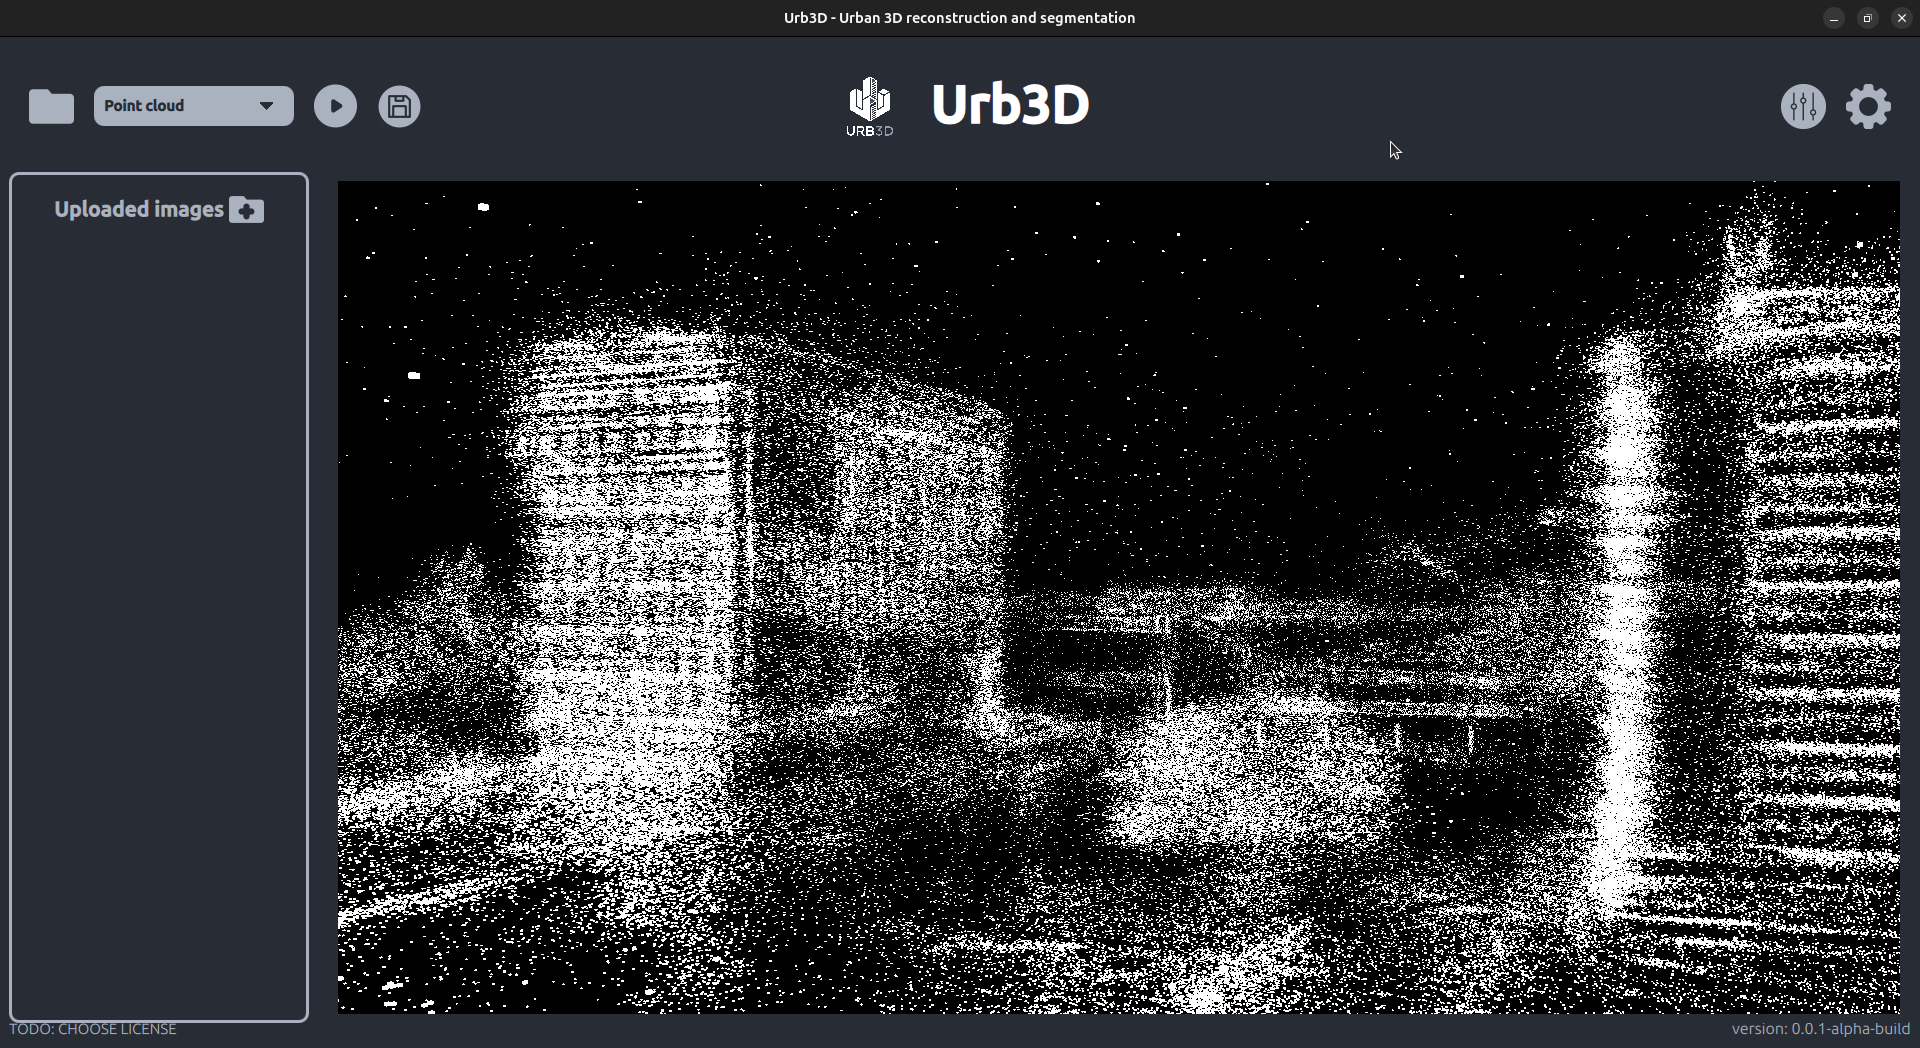
\includegraphics[width=0.8\textwidth]{img/wizualizacja/ui_rendering.png}
    \caption{Widok główny aplikacji z zaimplementowanym renderingiem.}
    \label{fig:widok_glowny}
\end{figure}

\subsubsection{Integracja z Pythonem}
Rendering został udostępniony jako dynamiczna biblioteka współdzielona, co umożliwia jego integrację z aplikacjami napisanymi w języku Python. Dzięki temu, w połączeniu z frameworkiem PyQt, rendering może być efektywnie wykorzystywany w aplikacjach graficznych.

\begin{figure}[h!]
    \centering
    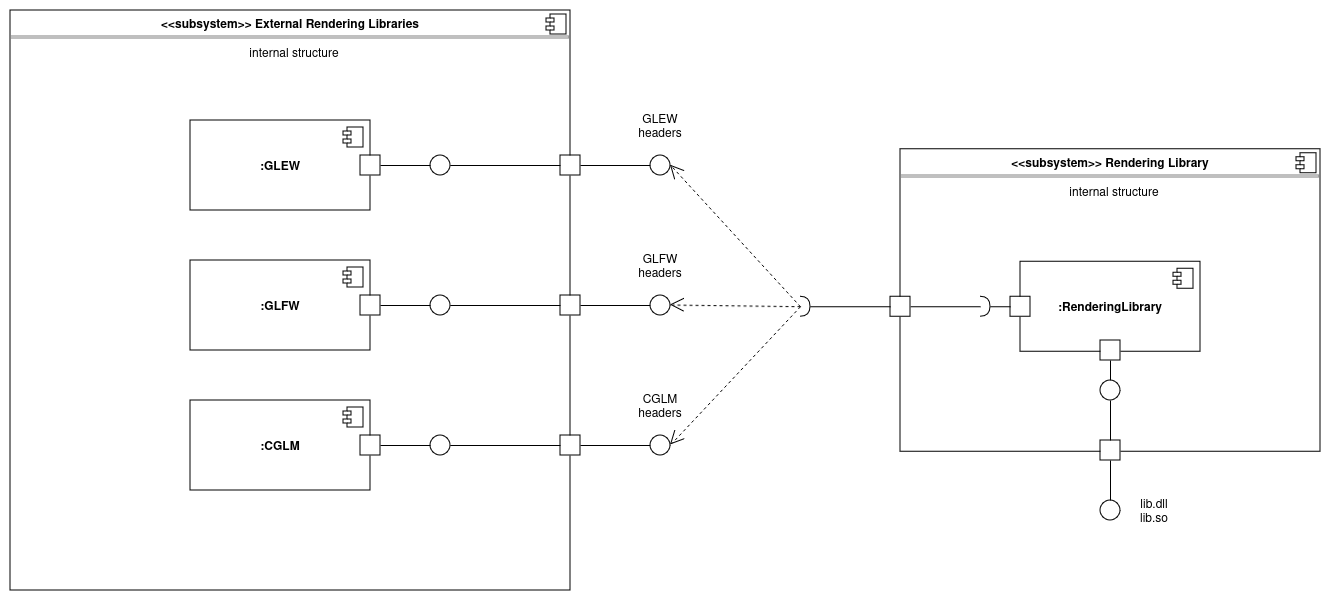
\includegraphics[width=0.8\textwidth]{img/diagramy/diagram_komp_rendering.png}
    \caption{Diagram przedstawiający architekturę integracji renderingu z Pythonem.}
    \label{fig:diagram}
\end{figure}

\subsubsection{Implementacja systemu renderingu}

\textbf{Reprezentacja punktów i splatów}
Wizualizacja punktów oraz splatów została zrealizowana za pomocą sześcianów, które są skalowane i rotowane w taki sposób, aby przypominały elipsoidy. Przetworzone w ten sposób sześciany są następnie renderowane przy użyciu shaderów, co pozwala na uzyskanie efektu ich zaokrąglenia.

\textbf{Optymalizacja wydajności}
Aby zwiększyć wydajność obliczeń graficznych, wykorzystano GPU z użyciem obiektów SSBO (Shader Storage Buffer Objects). SSBO umożliwiają przechowywanie i przetwarzanie dużych ilości danych bezpośrednio na karcie graficznej, co minimalizuje obciążenie procesora głównego.

W ramach procesu renderingu wczytywane są dane statyczne dla domyślnego sześcianu, a następnie przetwarzane są atrybuty poszczególnych punktów, takie jak:
\begin{itemize}
    \item pozycja,
    \item skalowanie,
    \item rotacja,
    \item przezroczystość,
    \item kolor.
\end{itemize}

Takie podejście zapewnia elastyczność oraz wysoką wydajność w generowaniu scen 3D.